\documentclass[11pt,a4paper,german,titlepage,oneside]{scrbook}
% ***** BEGIN OF THE LATEX PREAMBLE *****

\usepackage{amsmath}
\usepackage{amssymb}
\usepackage{bm} % Optional für fettgedruckte mathematische Symbole
\usepackage{softeng}
\usepackage{booktabs} % Ermöglicht \toprule, \midrule, \bottomrule
\usepackage{float}

\makeindex

\definecolor{lightgray}{gray}{0.9}

% Here we define the title of the current thesis in an appropriate variable.
\newcommand{\worktitle}{{\Huge SignNet}}
% Here we can define a subtitle for the work. If there is no subtitle let this variable empty.
\newcommand{\worksubtitle}{Gebärdensprachübersetzung mit Computer Vision \& Deep Learning}
% otherwise you can set any subtitle you want, event long ones by breaking the lines manually:
%\newcommand{\worksubtitle}{}
			   
% This is the name of the author
\newcommand{\theauthor}{\Large Andrei Chirilă \\ Roman Schläpfer}

% This command defines the type of the work: Master Thesis / Bachelor Thesis
\newcommand{\worktype}{Abschlussarbeit CAS Machine Learning for Software Engineers (ML4SE)}
% Date of the beginning of the work.

% Date of the end (submission) of the work.
\newcommand{\workdateyear}{2026}
\newcommand{\workdatemonth}{Januar}
\newcommand{\supervisorslabel}{Unter der Aufsicht von}

\newcommand{\worksupervisors}{
    Martin \textsc{Stypinski}\\
    Kursleiter CAS ML4SE\\
}

\newcommand{\titlepagefooter}{\titlepagefooterD}



% Here you define the labels of figures, tables, listings...
% English: Figure, Table, Listing (default)
% German: Abbildung, Tabelle, Listing
% French: Figure, Table, Listing
\renewcommand{\figurename}{Abbildung}
\renewcommand{\tablename}{Tabelle}
\renewcommand{\lstlistingname}{Listing} % default = Listing


% Let us set the path where all the figures have to be.
\graphicspath{{./figures/}}

% The following command avoids the indentation of the first sentence of each paragraph.
\parindent=0in

% The following command sets the header and footer style of the pages.
\pagestyle{fancy}

% The web resources are references in a bibliography apart.
\newcites{web}{Web Ressourcen}

% It is not mandatory (but suitable) to make an index. If you do not build an index: comment the line below!
% building the idx index file. This file is then to be compiled with %
% makeindex in the command line %
\usepackage{makeidx} \makeindex

% XML LstListing language settings







% ***** END OF THE LATEX PREAMBLE *****

% ***** BEGIN OF THE DOCUMENT *****
% ----- BEGIN OF THE FRONT STUFF -----
\begin{document}
% This line generates mini table of contents (tocs) at the beginning of each chapter, [e] for empty title.
\dominitoc[e] 
\pagestyle{empty}

% Here we include the titlepage.
\include{titlepage}

% The first pages are numbered in roman style.
\pagenumbering{roman}
\pagestyle{headings} 

% Now we include the abstract of you work
%\chapter*{Acknowledgements}

I also want to thank all the people that helped me, provided me with food, shelter, good discussions and a lot more during the long nights of coding. Thank you for everything.

\chapter*{Abstract}
\label{ch:abstract}

Diese Arbeit untersucht den Einsatz von Transformer-Modellen zur automatisierten Erkennung von Gebärdensprache anhand von Landmark-Sequenzen, die mit MediaPipe extrahiert wurden. Ziel war die Entwicklung eines robusten Klassifikators, der mit Klassenimbalance und visuellen Ähnlichkeiten umgehen kann. Als Datengrundlage dient der PHOENIX-Datensatz, ergänzt durch abgeleitete Merkmale wie Geschwindigkeits- und Knochenvektoren. Die Methodik kombiniert gezieltes Feature-Engineering mit einer angepassten Transformer-Architektur und einer hierarchischen Inferenzstrategie. Die Experimente zeigen eine deutliche Steigerung der Genauigkeit gegenüber Standardarchitekturen und eine höhere Fehlertoleranz bei seltenen Klassen. Abschließend werden die wichtigsten Fehlerquellen analysiert und Ansätze zur Verbesserung diskutiert. Die Ergebnisse liefern Impulse für zukünftige Forschung und praktische Anwendungen in der Gebärdensprachübersetzung.


% In order to have all references in your bibtex files figuring in the bibliorgraphy you can uncomment following lines.
% Otherwise, only the cited references will appear in your bibliography.
\nocite{*}
\nociteweb{*}

\begin{spacing}{1.0}  % Environment for 1.2 line spacing for contents and lists

% Here comes the table of contents
% Setting the name of the table of contents
%\renewcommand{\contentsname}{Table of Contents}  % Original name = Contents
\tableofcontents    % table of contents (.toc file) -- to rename title \renewcommand{\contentsname}{Table of Contents}

% Here comes the list of figures
% \listoffigures    % list of figures   (.lof file) -- to rename title \renewcommand{\listfigurename}{Figures}

% Here comes the list of tables
% \listoftables    % list of tables    (.lot file) -- to rename title \renewcommand{\listtablename}{Tables}

% Here comes the list of listings/code extracts
% Setting the name of the table of listings
% \lstlistoflistings    % list of listings    (.lol file) -- to rename title \renewcommand{\listtablename}{Tables}

\end{spacing}  % Environment for 1.2 line spacing for contents and lists

% ----- END OF THE FRONT STUFF -----

% ----- BEGIN OF THE MAIN BODY OF THE DOCUMENT -----

% Page numbering will now be arabic.
\pagenumbering{arabic}

\addtolength{\parskip}{0.1\baselineskip} % paragraph spacing

%\chapter*{Abstract}
\label{ch:abstract}

Diese Arbeit untersucht den Einsatz von Transformer-Modellen zur automatisierten Erkennung von Gebärdensprache anhand von Landmark-Sequenzen, die mit MediaPipe extrahiert wurden. Ziel war die Entwicklung eines robusten Klassifikators, der mit Klassenimbalance und visuellen Ähnlichkeiten umgehen kann. Als Datengrundlage dient der PHOENIX-Datensatz, ergänzt durch abgeleitete Merkmale wie Geschwindigkeits- und Knochenvektoren. Die Methodik kombiniert gezieltes Feature-Engineering mit einer angepassten Transformer-Architektur und einer hierarchischen Inferenzstrategie. Die Experimente zeigen eine deutliche Steigerung der Genauigkeit gegenüber Standardarchitekturen und eine höhere Fehlertoleranz bei seltenen Klassen. Abschließend werden die wichtigsten Fehlerquellen analysiert und Ansätze zur Verbesserung diskutiert. Die Ergebnisse liefern Impulse für zukünftige Forschung und praktische Anwendungen in der Gebärdensprachübersetzung.
\chapter{Einleitung}

\section{Thematik und Relevanz}
Gebärdensprachen sind vollwertige, natürliche Sprachen mit eigener Grammatik und Syntax, die von Millionen gehörloser und schwerhöriger Menschen weltweit als primäres Kommunikationsmittel verwendet werden. Die Kommunikation zwischen Gehörlosen und Hörenden stellt jedoch im Alltag oft eine erhebliche Barriere dar, da nur ein Bruchteil der hörenden Bevölkerung die Gebärdensprache beherrscht. Trotz der signifikanten Anzahl an Gebärdensprachnutzern fehlt es an barrierefreien Kommunikationslösungen in vielen Bereichen des täglichen Lebens – von öffentlichen Einrichtungen über Gesundheitswesen bis hin zu Bildungseinrichtungen.

Die automatische Erkennung von Gebärdensprach-Glossen (Automatic Sign Language Recognition, ASLR) bietet das Potenzial, diese Kommunikationslücke durch technologiegestützte Übersetzungssysteme zu schließen. Fortschritte in den Bereichen Computer Vision und Deep Learning haben in den letzten Jahren neue Möglichkeiten eröffnet, visuelle Informationen aus Videosequenzen zu extrahieren und zu klassifizieren.

\section{Problemstellung}
Die Komplexität der Gebärdensprache liegt in ihrer Multimodalität: Informationen werden simultan über Handbewegungen, Handformen, Körperhaltung und Mimik übertragen. Eine einzelne Gebärde kann aus der Kombination von bis zu fünf simultanen Parametern bestehen – Handform, Handstellung, Ausführungsstelle, Bewegung und non-manuelle Komponenten wie Gesichtsausdruck.

Technisch resultiert dies in hochdimensionalen, zeitlich variablen Datenströmen. Die Extraktion relevanter Merkmale aus Videosequenzen erfordert sowohl räumliche als auch temporale Modellierung. Während ein einzelnes Videoframe bereits hunderte von Landmark-Koordinaten (Hände, Körper, Gesicht) enthält, müssen diese über variable Sequenzlängen hinweg analysiert werden.

Zudem leiden aktuelle Datensätze unter einer ausgeprägten \textit{Long-Tail}-Verteilung: Wenige häufige Begriffe dominieren, während die Mehrheit der Gebärden nur selten vorkommt. Diese Klassenungleichheit erschwert das Training tiefer neuronaler Netze erheblich, da Modelle dazu tendieren, seltene Klassen zu vernachlässigen.

Ein weiteres Problem ist die hohe Ähnlichkeit zwischen bestimmten Gebärdengruppen. Richtungsangaben (Nord, Süd, Ost, West) oder semantisch verwandte Begriffe (verschiedene Wetterphänomene) unterscheiden sich oft nur in subtilen Bewegungsdetails, was zu systematischen Verwechslungen führt.

\section{Zielsetzung}
Das Hauptziel dieser Arbeit ist die Entwicklung, Implementierung und Evaluation des \textit{SignNet}-Systems zur Erkennung von Gebärdensprach-Glossen. Im Zentrum steht die Frage, ob ein hierarchisches Klassifikationsverfahren die Erkennungsgenauigkeit gegenüber einem monolithischen Ansatz verbessern kann.

Konkret werden folgende Ziele verfolgt:

\begin{itemize}
    \item \textbf{Entwicklung einer robusten Feature-Extraction-Pipeline}: Extraktion von Körper-, Hand- und Gesichtslandmarks mittels MediaPipe und deren Aufbereitung für maschinelles Lernen.
    \item \textbf{Implementierung eines Transformer-basierten Klassifikators}: Nutzung von Attention-Mechanismen zur Modellierung temporaler Abhängigkeiten in Gebärdensequenzen.
    \item \textbf{Hierarchische Expertenmodelle}: Entwicklung spezialisierter Submodelle für systematisch verwechselte Gebärdengruppen (z.B. Richtungsangaben, Wetterbegriffe).
    \item \textbf{Umgang mit Klassenungleichheit}: Evaluation verschiedener Strategien wie Focal Loss, Balanced Softmax und Oversampling.
    \item \textbf{Evaluation auf dem Phoenix-Datensatz}: Quantitative Bewertung der Erkennungsleistung auf einem etablierten Benchmark für Deutsche Gebärdensprache.
\end{itemize}

Die Arbeit soll demonstrieren, inwieweit aktuelle Deep-Learning-Methoden für die praktische Anwendung in der Gebärdenerkennung geeignet sind und welche architektonischen Entscheidungen die Klassifikationsgenauigkeit beeinflussen.

\chapter{Stand der Technik}
\label{ch:state_of_the_art}

Die automatische Gebärdenspracherkennung (Isolated Sign Recognition) hat in den letzten Jahrzehnten eine signifikante Entwicklung durchlaufen, die von handgesteuerten statistischen Modellen hin zu komplexen Deep-Learning-Architekturen reicht \cite{1}.

\section{Traditionelle Methoden und frühes Machine Learning}
Vor dem Aufkommen von Deep Learning basierten Systeme primär auf handgefertigten Merkmalen (Hand-crafted Features), wie etwa relativen Handpositionen oder Distanzen zwischen Händen und spezifischen Körperteilen \cite{46}. Zur Klassifizierung dieser raumzeitlichen Informationen wurden klassische Algorithmen wie Hidden Markov Models (HMMs), Conditional Random Fields (CRFs), Support Vector Machines (SVMs) und k-Nearest Neighbors (kNNs) eingesetzt \cite{35, 46}. Ein wesentlicher Nachteil dieser Ansätze war jedoch ihre begrenzte Generalisierungsfähigkeit und Skalierbarkeit aufgrund der zugrunde liegenden Gaußschen Verteilungsannahmen \cite{47}.

\section{RGB-basierte Deep-Learning-Ansätze}
Mit dem Durchbruch neuronaler Netze verschob sich der Fokus auf die Extraktion von Merkmalen direkt aus Videodaten.

\subsection{CNN-RNN Architekturen}
Frühe Deep-Learning-Modelle kombinierten Convolutional Neural Networks (CNNs) zur Extraktion räumlicher Merkmale in jedem Frame mit rekurrenten Netzwerken wie LSTMs oder Bidirectional LSTMs (Bi-LSTMs), um die zeitliche Dynamik der Gebärden zu erfassen \cite{53, 69}.

\subsection{3D-CNNs und zeitliche Modellierung}
Um kurzfristige zeitliche Abhängigkeiten besser abzubilden, wurden 3D-CNNs eingeführt, wobei das Inflated 3D-CNN (I3D) zu einer der am häufigsten verwendeten Architekturen wurde \cite{55, 57}. Diese Modelle verbessern das Lernen zeitlicher Merkmale, weisen jedoch Schwächen bei der Erfassung langfristiger Abhängigkeiten auf, da diese oft auf die finale globale Durchschnittspooling-Stufe beschränkt sind \cite{58}.

\subsection{Transformer und Attention-Mechanismen}
In jüngster Zeit werden vermehrt Transformer-Modelle eingesetzt, die den Self-Attention-Mechanismus nutzen \cite{61}. Diese haben den Vorteil, raumzeitliche Abhängigkeiten über das gesamte Video hinweg zu erfassen \cite{63}. Ein kritischer Faktor bleibt hierbei jedoch der hohe Bedarf an großen Mengen an Trainingsdaten, die in der Gebärdensprachforschung oft nur begrenzt zur Verfügung stehen \cite{64}.

\section{Skelettbasierte Ansätze}
Anstatt rohe RGB-Frames zu verwenden, nutzen skelettbasierte Methoden extrahierte Keypoints von Gelenken, um das Lernen auf relevante Bewegungsinformationen zu fokussieren und Hintergrundrauschen zu eliminieren \cite{66, 67}.

\subsection{Graph Convolutional Networks (GCN)}
Das Spatial-Temporal Graph Convolutional Network (ST-GCN) markierte einen wichtigen Fortschritt bei der Modellierung der raumzeitlichen Dynamik von Skeletten \cite{71}. Frühe GCN-Modelle verarbeiteten Informationen jedoch oft nur entlang der natürlichen biologischen Verbindungen des menschlichen Körpers, wodurch Interaktionen zwischen nicht direkt verbundenen Punkten (z. B. zwischen den beiden Händen) weitgehend ignoriert wurden \cite{72, 73}. Neuere Ansätze versuchen dies durch adaptive Graphen oder Multi-Stream-Modelle zu kompensieren \cite{75, 76}.

\section{Multimodale Fusion und aktuelle Entwicklungen}
Der aktuelle Stand der Technik wird durch die Kombination mehrerer Merkmalsströme (Multi-feature Combination) definiert. Hierbei werden Informationen aus RGB-Videos, extrahierten 2D/3D-Skeletten, optischem Fluss und Tiefendaten fusioniert \cite{81, 83}. Moderne Frameworks erreichen so Top-1-Genauigkeiten von über 77\% auf modifizierten WLASL-Datensätzen, indem sie bidirektionale Datenströme und eine explizite Erkennung der Start- und Endframes von Gebärden nutzen \cite{15, 16, 39, 40}. Insbesondere die Konsistenz der Gloss-Labeling-Konventionen (1-zu-1-Korrespondenz zwischen Gebärde und Textlabel) hat sich als entscheidend für die Leistungsfähigkeit der Modelle erwiesen \cite{14, 95}.

\chapter{Hintergrund}
\label{ch:background}

Dieses Kapitel führt in die theoretischen Grundlagen ein, die für das Verständnis der vorliegenden Arbeit notwendig sind. Zunächst wird die Gebärdensprache als linguistisches System vorgestellt, gefolgt von den technischen Grundlagen der verwendeten Deep-Learning-Architektur und der Merkmalsextraktion.

\section{Gebärdensprache als linguistisches System}

Gebärdensprachen sind vollwertige, natürliche Sprachen mit eigener Grammatik, Syntax und Morphologie. Im Gegensatz zu weit verbreiteten Missverständnissen handelt es sich nicht um eine visuelle Kodierung gesprochener Sprache oder um Pantomime, sondern um eigenständige linguistische Systeme \cite{stokoe1960}.

\subsection{Phonologie der Gebärdensprache}

William Stokoe legte 1960 den Grundstein für die linguistische Analyse von Gebärdensprachen, indem er nachwies, dass Gebärden – analog zu gesprochenen Wörtern – aus kleineren, bedeutungsunterscheidenden Einheiten bestehen. Diese Einheiten werden als \textit{Cheremes} (in Anlehnung an Phoneme) oder heute häufiger als \textit{Parameter} bezeichnet.

Eine Gebärde setzt sich aus fünf simultanen Parametern zusammen:

\begin{itemize}
    \item \textbf{Handform}: Die Konfiguration der Finger (z.B. flache Hand, Faust, ausgestreckter Zeigefinger). Die Deutsche Gebärdensprache (DGS) verwendet etwa 30 distinktive Handformen.
    \item \textbf{Handstellung (Orientierung)}: Die Ausrichtung der Handfläche und Finger relativ zum Körper (z.B. Handfläche nach oben, nach unten, zum Körper).
    \item \textbf{Ausführungsort}: Die Position im Gebärdenraum, an der die Gebärde ausgeführt wird (z.B. vor der Brust, am Kopf, im neutralen Raum).
    \item \textbf{Bewegung}: Die Art und Richtung der Handbewegung (z.B. linear, kreisförmig, wiederholend).
    \item \textbf{Non-manuelle Komponenten}: Mimik, Mundbild, Kopf- und Körperhaltung, die grammatische oder lexikalische Informationen tragen.
\end{itemize}

Diese Simultaneität unterscheidet Gebärdensprachen fundamental von sequentiell aufgebauten Lautsprachen und stellt besondere Anforderungen an maschinelle Erkennungssysteme.

\subsection{Glossennotation}

In der Gebärdensprachforschung werden Gebärden typischerweise durch \textit{Glossen} repräsentiert – konventionalisierte Bezeichnungen in Großbuchstaben, die auf der Bedeutung der Gebärde basieren. Die Glosse \texttt{HAUS} bezeichnet beispielsweise die Gebärde für das Konzept "Haus", unabhängig von der spezifischen Ausführungsform. Diese Notation ermöglicht die Annotation von Videodaten und bildet die Grundlage für überwachtes maschinelles Lernen.

\subsection{Isolierte vs. kontinuierliche Gebärdenerkennung}

Man unterscheidet zwei Hauptaufgaben in der automatischen Gebärdenerkennung:

\begin{itemize}
    \item \textbf{Isolierte Gebärdenerkennung (Isolated Sign Language Recognition, ISLR)}: Klassifikation einzelner, segmentierter Gebärden. Der Anfang und das Ende der Gebärde sind bekannt.
    \item \textbf{Kontinuierliche Gebärdenerkennung (Continuous Sign Language Recognition, CSLR)}: Erkennung von Gebärdensequenzen ohne vorgegebene Segmentierung, analog zur Spracherkennung.
\end{itemize}

Die vorliegende Arbeit fokussiert sich auf die isolierte Gebärdenerkennung, bei der vorgeschnittene Videosequenzen einzelnen Glossen zugeordnet werden.

\section{Transformer-Architektur}

Die Transformer-Architektur \cite{vaswani2017} hat sich als dominantes Paradigma für die Verarbeitung sequentieller Daten etabliert. Im Gegensatz zu rekurrenten Netzwerken (RNNs, LSTMs) verarbeitet der Transformer die gesamte Sequenz parallel und modelliert Abhängigkeiten durch einen Attention-Mechanismus.

\subsection{Self-Attention}

Der Kern des Transformers ist der \textit{Self-Attention}-Mechanismus, der es jedem Element einer Sequenz ermöglicht, Informationen von allen anderen Elementen zu aggregieren. Für eine Eingabesequenz $\mathbf{X} \in \mathbb{R}^{T \times d}$ mit $T$ Zeitschritten und Dimension $d$ werden drei Projektionen berechnet:

\begin{align}
    \mathbf{Q} &= \mathbf{X} \mathbf{W}^Q \quad \text{(Queries)} \\
    \mathbf{K} &= \mathbf{X} \mathbf{W}^K \quad \text{(Keys)} \\
    \mathbf{V} &= \mathbf{X} \mathbf{W}^V \quad \text{(Values)}
\end{align}

Die Attention-Gewichte werden durch Skalierung des Skalarprodukts zwischen Queries und Keys berechnet:

\begin{equation}
    \text{Attention}(\mathbf{Q}, \mathbf{K}, \mathbf{V}) = \text{softmax}\left(\frac{\mathbf{Q}\mathbf{K}^\top}{\sqrt{d_k}}\right) \mathbf{V}
\end{equation}

Durch diesen Mechanismus kann jeder Frame einer Gebärdensequenz Informationen von allen anderen Frames berücksichtigen, was besonders für die Erfassung globaler Bewegungsmuster relevant ist.

\subsection{Positional Encoding}

Da der Transformer keine inhärente Sequenzordnung besitzt, muss die zeitliche Position explizit kodiert werden. Dies geschieht durch \textit{Positional Encodings}, die zur Eingabe addiert werden. In dieser Arbeit werden \textit{lernbare} Positional Embeddings verwendet, die während des Trainings optimiert werden:

\begin{equation}
    \mathbf{X}' = \mathbf{X} + \mathbf{E}_{\text{pos}}
\end{equation}

wobei $\mathbf{E}_{\text{pos}} \in \mathbb{R}^{T_{\max} \times d}$ eine trainierbare Embedding-Matrix ist.

\subsection{Vorteile gegenüber rekurrenten Architekturen}

Transformer bieten mehrere Vorteile für die Gebärdenerkennung:

\begin{itemize}
    \item \textbf{Parallelisierung}: Alle Positionen werden gleichzeitig verarbeitet, was das Training beschleunigt.
    \item \textbf{Lange Abhängigkeiten}: Direkte Verbindungen zwischen beliebigen Positionen vermeiden das Problem verschwindender Gradienten bei langen Sequenzen.
    \item \textbf{Interpretierbarkeit}: Attention-Gewichte können visualisiert werden, um zu verstehen, welche Frames für die Klassifikation relevant sind.
\end{itemize}

\section{Herausforderungen des Datensatzes}

\subsection{Long-Tail-Verteilung}

Ein zentrales Problem der Gebärdenspracherkennung ist die ungleiche Verteilung der Trainingsbeispiele. Der verwendete Phoenix-Datensatz folgt einer \textit{Power-Law}-Verteilung: Wenige häufige Gebärden (z.B. \texttt{REGION}, \texttt{MORGEN}) dominieren, während die Mehrheit der Klassen nur selten vorkommt.

\subsection{Gini-Koeffizient}

Die Ungleichverteilung lässt sich durch den Gini-Koeffizienten $G$ quantifizieren. Für $n$ Klassen mit den jeweiligen Stichprobenanzahlen $x_i$ gilt:

\begin{equation}
    G = \frac{\sum_{i=1}^n \sum_{j=1}^n |x_i - x_j|}{2n \sum_{i=1}^n x_i}
\end{equation}

Ein hoher Gini-Koeffizient deutet auf eine extreme Konzentration der Daten auf wenige "Head-Klassen" hin, während die Mehrheit der Klassen ("Tail") unterrepräsentiert ist. Dies erfordert spezielle Trainingsstrategien wie Focal Loss, Class-Balanced Loss oder Oversampling.

\subsection{Visuelle Konfusion}

Zusätzlich zur statistischen Imbalance erschwert die \textit{phonologische Ähnlichkeit} die Klassifikation. Viele Gebärden unterscheiden sich lediglich in einem Parameter – beispielsweise unterscheiden sich die Gebärden für Himmelsrichtungen (\texttt{NORD}, \texttt{SUED}, \texttt{OST}, \texttt{WEST}) primär durch die Bewegungsrichtung bei ansonsten identischer Handform und -position.

Solche systematisch verwechselten Gruppen werden in dieser Arbeit als \textit{Konfusionscluster} bezeichnet. Sie motivieren die Implementierung hierarchischer Expertenmodelle, die auf die Unterscheidung innerhalb spezifischer Cluster spezialisiert sind.

\chapter{Methodik}
\label{ch:methodology}

Dieses Kapitel beschreibt die technische Umsetzung und den iterativen Forschungsprozess des \textit{SignNet}-Systems. Im Mittelpunkt steht die Begründung der Designentscheidungen, die in fünf aufeinanderfolgenden Entwicklungsphasen getroffen wurden, um eine robuste und dynamische Gebärdenspracherkennung zu realisieren.

\section{Datengrundlage und Klassenwahl}
Die Basis für die dynamische Erkennung bildet der \textit{Phoenix}-Datensatz, der ursprünglich über 1200 verschiedene Gebärden (Glossen) umfasst.

\subsection{Filterkriterien und Stichprobenumfang}
Da der Datensatz eine starke Klassenimbalance (Long-Tail-Verteilung) aufweist, wurde das Vokabular bewusst eingeschränkt, um die Robustheit des Trainings zu erhöhen:

\begin{itemize}
    \item \textbf{Mindestanforderung}: Es wurden nur Klassen berücksichtigt, die mindestens \texttt{MIN\_SAMPLES\_PER\_CLASS = 70} Beispiele enthalten.
    \item \textbf{Resultat}: Nach der Filterung blieben \textbf{146 Klassen} für die finale Klassifizierung übrig.
    \item \textbf{Begründung}: Diese Auswahl stellt sicher, dass das Modell pro Gebärde genügend Varianz erhält, um verallgemeinerbare Merkmale zu lernen und nicht nur auswendig zu lernen (Overfitting).
\end{itemize}

\subsection{Merkmalsextraktion mit MediaPipe}
Um die Komplexität der Rohvideodaten zu reduzieren und das System robust gegenüber variierenden Hintergründen und Lichtverhältnissen zu machen, wurde die \textit{MediaPipe}-Pipeline eingesetzt \cite{lugaresi2019}. Anstatt das Modell direkt auf Pixelebene zu trainieren, extrahiert diese Pipeline anatomisch relevante 3D-Landmarks aus jedem Frame der Videosequenz.

Die Extraktion erfolgt in drei spezialisierten Submodellen, deren Ergebnisse zu einem kombinierten Merkmalsvektor zusammengefasst werden:

\begin{itemize}
    \item \textbf{Face-Mesh}: 478 Landmarks für mimische Details und Mundbilder.
    \item \textbf{Hand-Tracking}: 21 Landmarks pro Hand (insgesamt 42 Punkte) für die präzise Fingerstellung.
    \item \textbf{Pose-Modell}: 33 Landmarks zur Definition der Oberkörperposition.
\end{itemize}

Insgesamt ergeben sich 553 Punkte, die jeweils durch ein Koordinatentripel $(x, y, z)$ repräsentiert werden. Das führt zu einer Eingabedimension von 1659 Merkmalen pro Frame. Dieser flache Merkmalsvektor dient als Grundlage für das anschließende Feature Engineering, wie die Berechnung von Geschwindigkeiten und Knochenvektoren. Dabei sind $x$ und $y$ auf die Bildbreite und -höhe normiert ($[0, 1]$), während $z$ die geschätzte Tiefe relativ zur Kamera darstellt.

\section{Iterativer Forschungsansatz und Versuchsaufbau}
Das finale System wurde nicht in einem Schritt entwickelt, sondern in fünf Etappen. Jede Phase basierte auf den Erkenntnissen der vorherigen und zielte darauf ab, Schwachstellen zu beheben.

\subsection{Phase 1: Statische Baseline (CNN) – Fingeralphabet}
In der ersten Phase wurde die Erkennung des statischen Fingeralphabets (25 Klassen) anhand von Bilddaten getestet:
\begin{itemize}
    \item \textbf{Designentscheidung}: Einsatz eines \textit{Convolutional Neural Networks} (CNN) zur direkten Merkmalsextraktion aus Pixeldaten.
    \item \textbf{Ergebnis}: Das Modell erreichte eine \textbf{Testgenauigkeit von 99,6\,\%}.
    \item \textbf{Erkenntnis}: Trotz der hohen Genauigkeit wurde klar, dass dieser Ansatz die zeitliche Dynamik der Gebärdensprache nicht erfassen kann.
\end{itemize}

\subsection{Phase 2: Erste dynamische Klassifizierung (150 Klassen)}
Die Erweiterung auf 150 dynamische Glossen erforderte den Wechsel von Einzelbildern zu Videosequenzen:
\begin{itemize}
    \item \textbf{Technischer Aufbau}: Nutzung von Landmark-Extraktionen zur Reduktion der Datenkomplexität.
    \item \textbf{Ergebnis}: Die Validierungsgenauigkeit lag bei \textbf{53,9\,\%}. Dies zeigte, dass herkömmliche Modelle bei steigender Klassenanzahl und zeitlicher Varianz an ihre Grenzen stoßen.
\end{itemize}

\subsection{Phase 3: Skelettbasierte Graph-Experimente}
Es wurde versucht, die anatomischen Relationen der Hand-Landmarks explizit durch skelettale Graphstrukturen abzubilden:
\begin{itemize}
    \item \textbf{Ergebnis}: Die Validierungsgenauigkeit sank deutlich auf \textbf{31,6\,\%}.
    \item \textbf{Designentscheidung}: Die Ergebnisse zeigten, dass starre skelettbasierte Graphen die hohe individuelle Variabilität in der Gebärdenausführung nicht ausreichend generalisieren konnten. Dies führte zur Entscheidung für eine flexiblere, auf Aufmerksamkeit basierende Architektur: den Transformer.
\end{itemize}

\subsection{Phase 4: Einführung der Transformer-Architektur}
Der Wechsel auf einen Transformer-Encoder markierte den technologischen Durchbruch für das Projekt:
\begin{itemize}
    \item \textbf{Konzept}: Implementierung eines \textit{Self-Attention}-Mechanismus, um zeitliche Abhängigkeiten über die gesamte Sequenz hinweg zu lernen.
    \item \textbf{Ergebnis}: Die Validierungsgenauigkeit stieg deutlich auf \textbf{66,6\,\%}.
\end{itemize}

\subsection{Phase 5: Finales optimiertes Modell}
Durch intensives Hyperparameter-Tuning und die Verfeinerung des Feature Engineerings wurde der aktuelle Bestwert erreicht:
\begin{itemize}
    \item \textbf{Optimierung}: Einführung von \textit{Label Smoothing} und optimierten kinematischen Features.
    \item \textbf{Resultat}: Das System erzielte eine finale \textbf{Validierungsgenauigkeit von 73,15\,\%} sowie eine \textbf{Top-5 Accuracy von 92,05\,\%}.
\end{itemize}

\section{Vorverarbeitung und Datenreinigung}
Ein robuster Umgang mit instabilen Datenquellen war entscheidend für die Modellstabilität.

\subsection{Umgang mit Fehlwerten und Verdeckungen (Occlusion)}
Die Landmark-Extraktion mittels MediaPipe ist anfällig für Verdeckungen, etwa wenn eine Hand die andere überschneidet:
\begin{itemize}
    \item \textbf{Numerische Stabilität}: Auftretende \texttt{NaN}-Werte werden in der Vorverarbeitung konsequent durch $0.0$ ersetzt, um Berechnungsfehler in den Transformer-Layern zu vermeiden.
    \item \textbf{Händigkeits-Invarianz}: Der \texttt{TransformerSignClassifierWithHandedness} erkennt explizit die dominante Hand, um die Vorhersage unabhängig von der Händigkeit des Unterzeichners zu machen.
\end{itemize}

\section{Datenaugmentation}
Um dem \textit{Long-Tail}-Problem des Datensatzes zu begegnen, wurde eine mehrstufige Augmentation implementiert.

\subsection{Spatiale und temporale Transformationen}
\begin{itemize}
    \item \textbf{Geometrischer Shift}: Zufällige Rotationen bis zu 5° und Skalierungen zwischen $0,9$ und $1,1$ simulieren variierende Kamerapositionen.
    \item \textbf{Temporaler Shift}: Sequenzen werden zufällig zeitlich verschoben, um die Invarianz gegenüber unterschiedlichen Startzeitpunkten einer Gebärde zu erhöhen.
\end{itemize}

\subsection{Landmark-Occlusion-Augmentation}
Zur Verbesserung der Robustheit gegenüber Verdeckungen wurde ein spezifisches Fehler-Modell integriert:
\begin{itemize}
    \item \textbf{Gaussian Noise}: Den Koordinaten wird ein normalverteiltes Rauschen ($\sigma = 0,005$) hinzugefügt.
    \item \textbf{Simulation von Jitter}: Dieses Rauschen simuliert die Instabilität der Keypoints, die typischerweise bei teilweisen Verdeckungen auftritt.
    \item \textbf{Lerneffekt}: Das Modell wird gezwungen, robuste Bewegungsmuster statt präziser Einzelpunkte zu lernen.
\end{itemize}

\section{Feature Engineering: Kinematik und Geometrie}
Die Klasse \texttt{EnhancedLandmarkFeatures} transformiert statische Punkte in einen dynamischen Merkmalsraum.

\subsection{Kinematische Ableitungen}
Die Bewegung wird durch Geschwindigkeit $\vec{v}_t$ und Beschleunigung $\vec{a}_t$ beschrieben, normiert durch die Bildrate (\textit{fps}):
\begin{equation}
    \vec{v}_t = (\mathbf{p}_t - \mathbf{p}_{t-1}) \cdot \text{fps} \quad , \quad \vec{a}_t = (\vec{v}_t - \vec{v}_{t-1}) \cdot \text{fps}
\end{equation}

\subsection{Skelett-Geometrie: Bone-Vektoren}
Um die Handform präzise abzubilden, werden Vektoren zwischen anatomisch verbundenen Gelenken berechnet:
\begin{equation}
    \vec{b} = \mathbf{p}_{\text{joint\_A}} - \mathbf{p}_{\text{joint\_B}}
\end{equation}
Diese Vektoren sind invariant gegenüber Translationen und erfassen die geometrische Konfiguration der Hand unabhängig von der Position im Bild.

\section{Modellarchitektur: Transformer-Encoder}
Die Wahl des Transformers begründet sich durch seine Fähigkeit, globale Abhängigkeiten effizient zu modellieren:
\begin{itemize}
    \item \textbf{Self-Attention}: Der Mechanismus erlaubt es dem Modell, irrelevante Phasen (z.\,B. das Heben der Hände) automatisch auszublenden und sich auf die linguistischen Kernbewegungen zu fokussieren.
    \item \textbf{Padding-Masking}: Mittels \texttt{PadCollate} und \texttt{seq\_lengths} werden variable Videolängen einheitlich verarbeitet, ohne dass Padding-Werte die Berechnung beeinflussen.
\end{itemize}

\subsection{Spezifikation der Transformer-Architektur}
Um Overfitting zu vermeiden, wurde für das finale Modell eine kompakte Transformer-Konfiguration gewählt. Die Modellgröße wurde gezielt reduziert, um eine bessere Generalisierung auf dem Validierungsset zu erreichen.

\begin{table}[h]
\centering
\caption{Hyperparameter der Transformer-Architektur (Phase 5)}
\label{tab:model_config}
\begin{tabular}{llp{11cm}}
\toprule
Parameter & Wert & Begründung \\
\midrule
\texttt{input\_size} & 1659 & Resultiert aus 553 Landmarks mit jeweils 3 Koordinaten ($x, y, z$). \\
\texttt{hidden\_size} & 256 & Reduktion von 512 auf 256 zur Vermeidung von Overfitting bei begrenzter Datenmenge. \\
\texttt{num\_layers} & 4 & Optimale Balance zwischen Rechentiefe und Trainingsstabilität (reduziert von 6 Layern). \\
\texttt{num\_heads} & 8 & Ermöglicht 8 parallele Attention-Heads mit jeweils 32 Dimensionen pro Head. \\
\texttt{dim\_feedforward} & 1024 & Entspricht dem 4-fachen der \texttt{hidden\_size} für ausreichende Kapazität im MLP-Block. \\
\bottomrule
\end{tabular}
\end{table}
\chapter{Resultate}
\label{ch:results}

In diesem Kapitel stellen wir die quantitativen Resultate aus den fünf Entwicklungsphasen vor. Die Daten stammen aus den MLflow-Tracking-Aufzeichnungen sowie den Evaluierungsläufen der jeweiligen Modellvarianten.

\section{Vergleich der Entwicklungsphasen}
Über den gesamten Projektverlauf hinweg haben wir die Performance der verschiedenen Modellarchitekturen systematisch erfasst. In \autoref{tab:phase_accuracy} sehen Sie, wie sich die Genauigkeit (Accuracy) von der statischen Vorphase bis hin zum finalen Transformer-Modell entwickelt hat.

\begin{table}[h]
\centering
\caption{Übersicht der erreichten Genauigkeiten pro Phase}
\label{tab:phase_accuracy}
\begin{tabular}{cllr}
\toprule
Phase & Architektur & Fokus & Validierungsgüte \\
\midrule
1 & CNN & Statisches Alphabet (25 Klassen) & 99,60 \% \\
2 & Transformer v1 & Dynamische Gebärden (146 Klassen) & 53,94 \% \\
3 & Skeleton-Graph & Anatomische Graphen-Pipeline & 31,56 \% \\
4 & Transformer v2 & Self-Attention Baseline & 66,61 \% \\
5 & Transformer Final & Optimiertes Feature Engineering & 73,86 \% \\
\bottomrule
\end{tabular}
\end{table}

\section{Analyse des Trainingsverlaufs}
Um die Stabilität und Konvergenz des finalen Modells (Phase 5) zu prüfen, haben wir den Verlauf von Loss und Accuracy während des Trainings aufgezeichnet.

\begin{figure}[htbp]
    \centering
    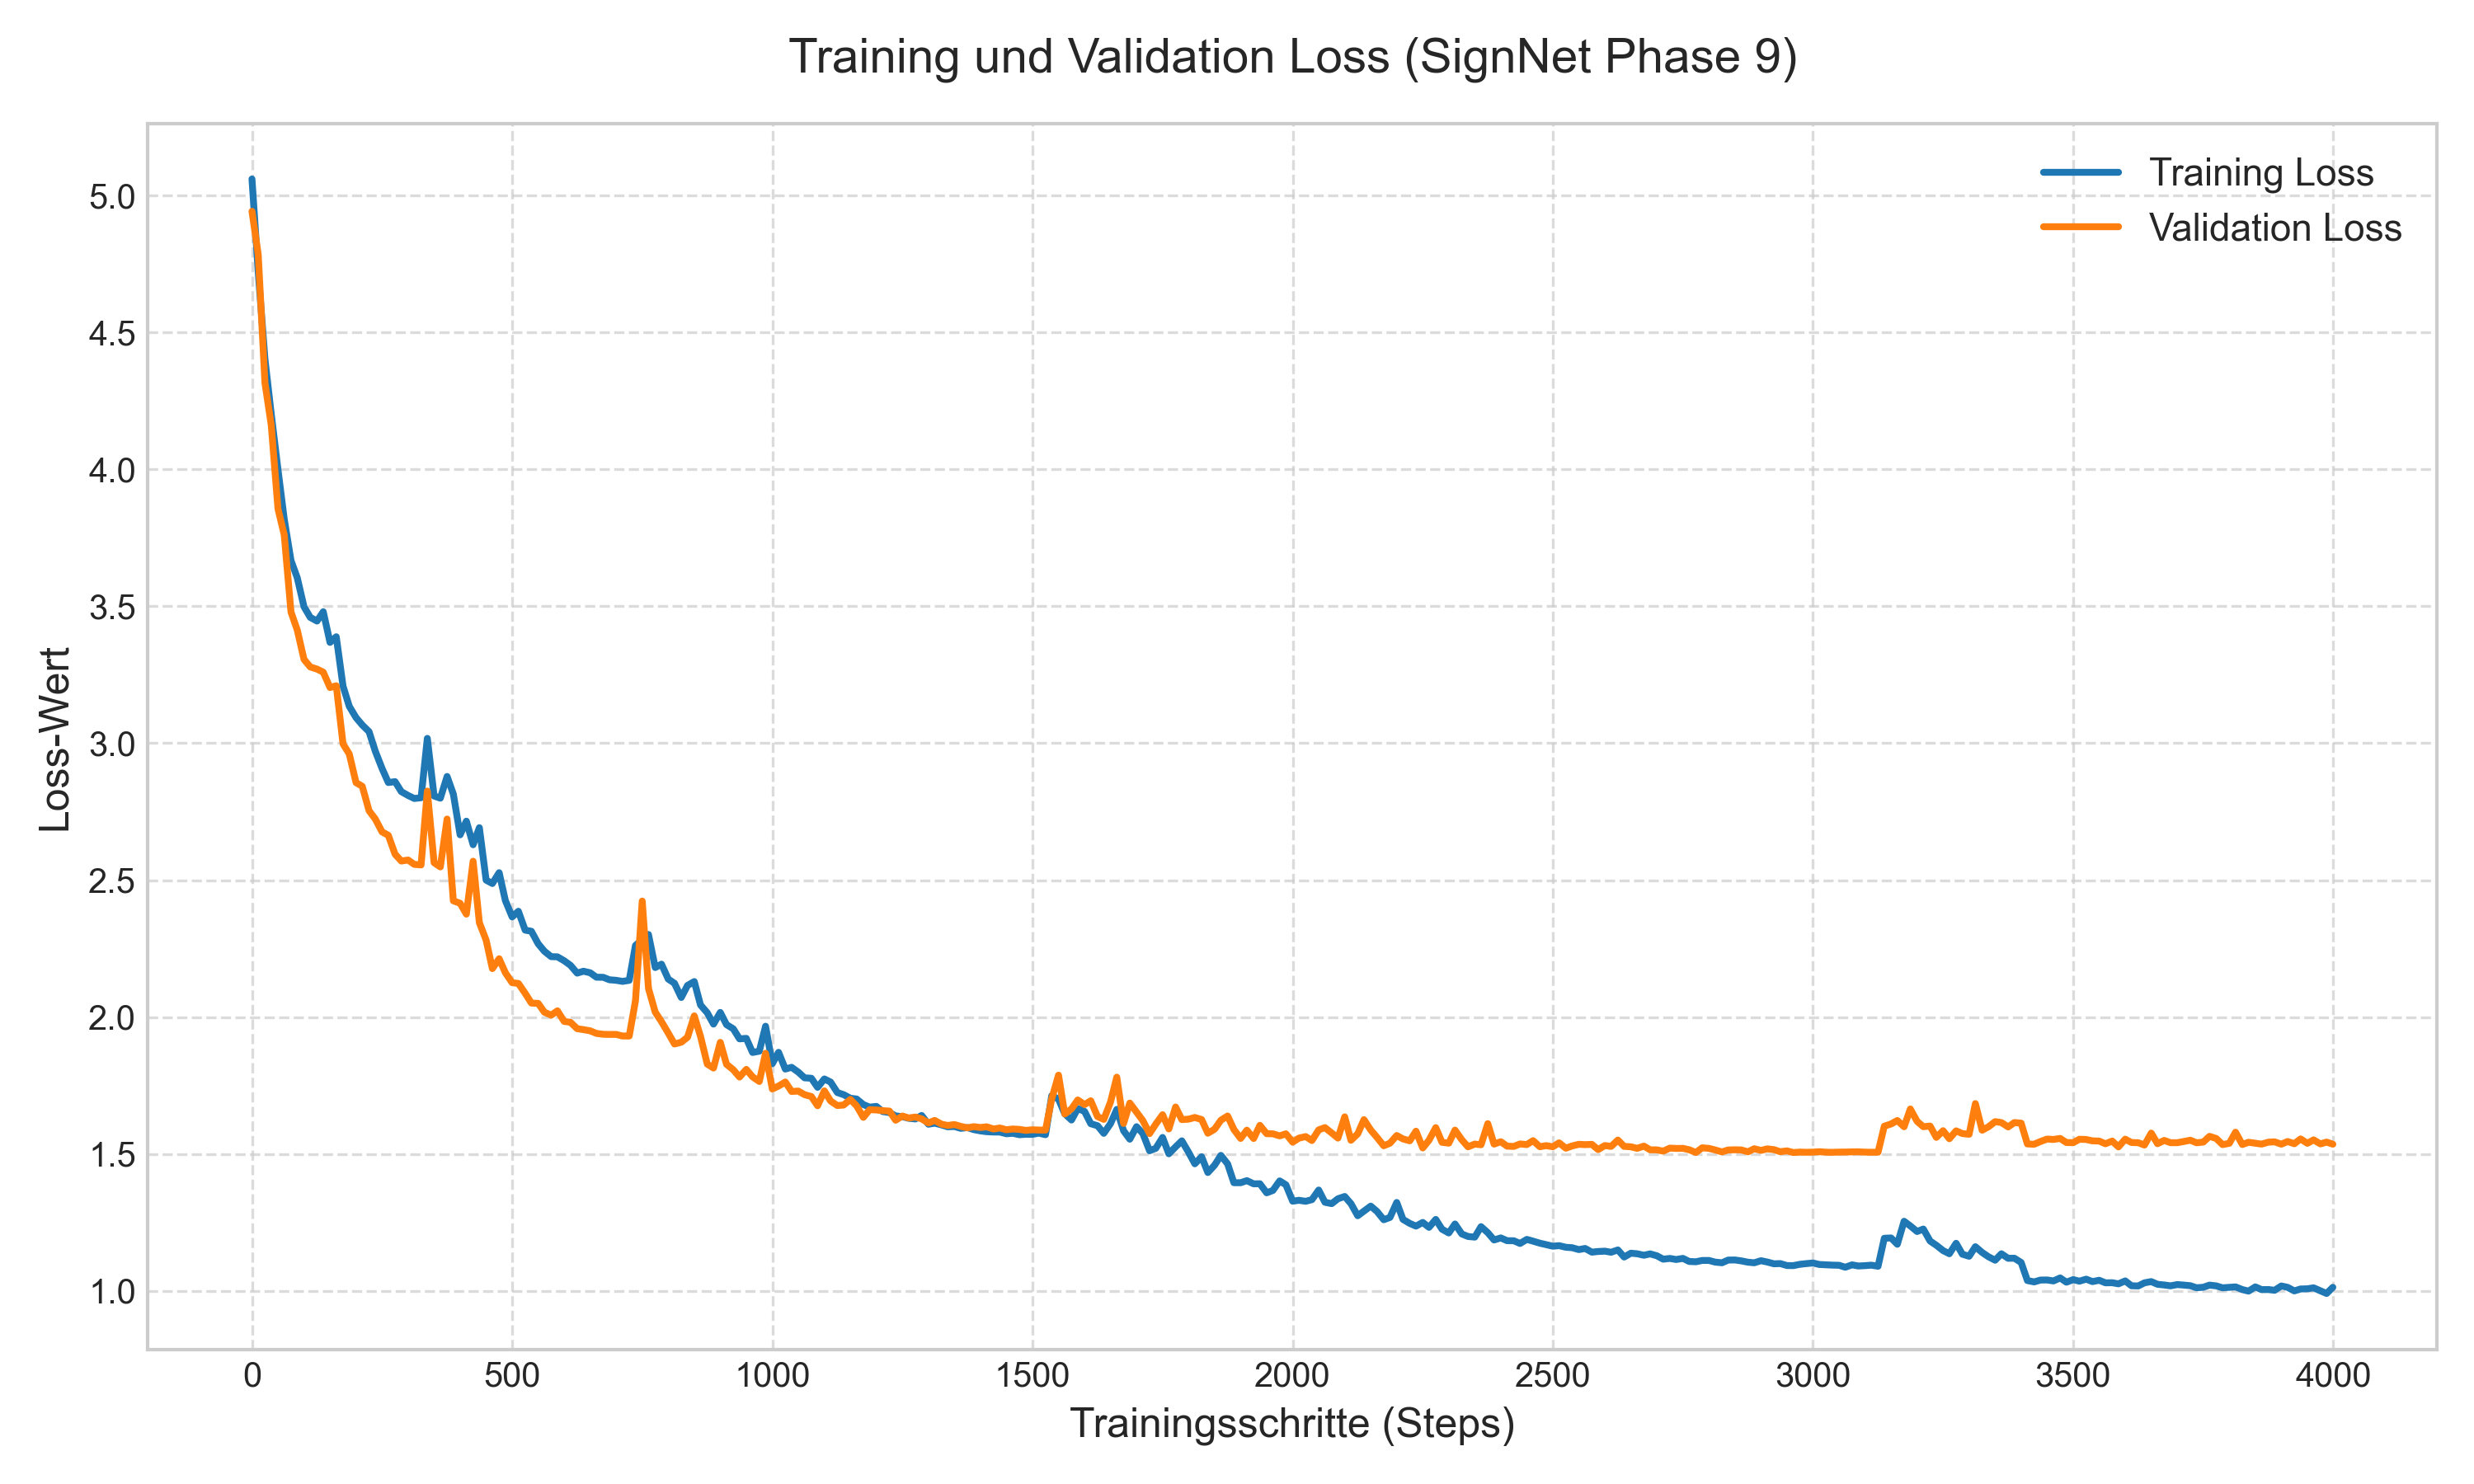
\includegraphics[width=0.85\textwidth]{figures/loss_plot_final.png}
    \caption{Verlauf von Trainings- und Validierungs-Loss: Die stetige Abnahme beider Kurven ohne Divergenz deutet auf eine gute Generalisierung hin.}
    \label{fig:loss_plot}
\end{figure}

\begin{figure}[htbp]
    \centering
    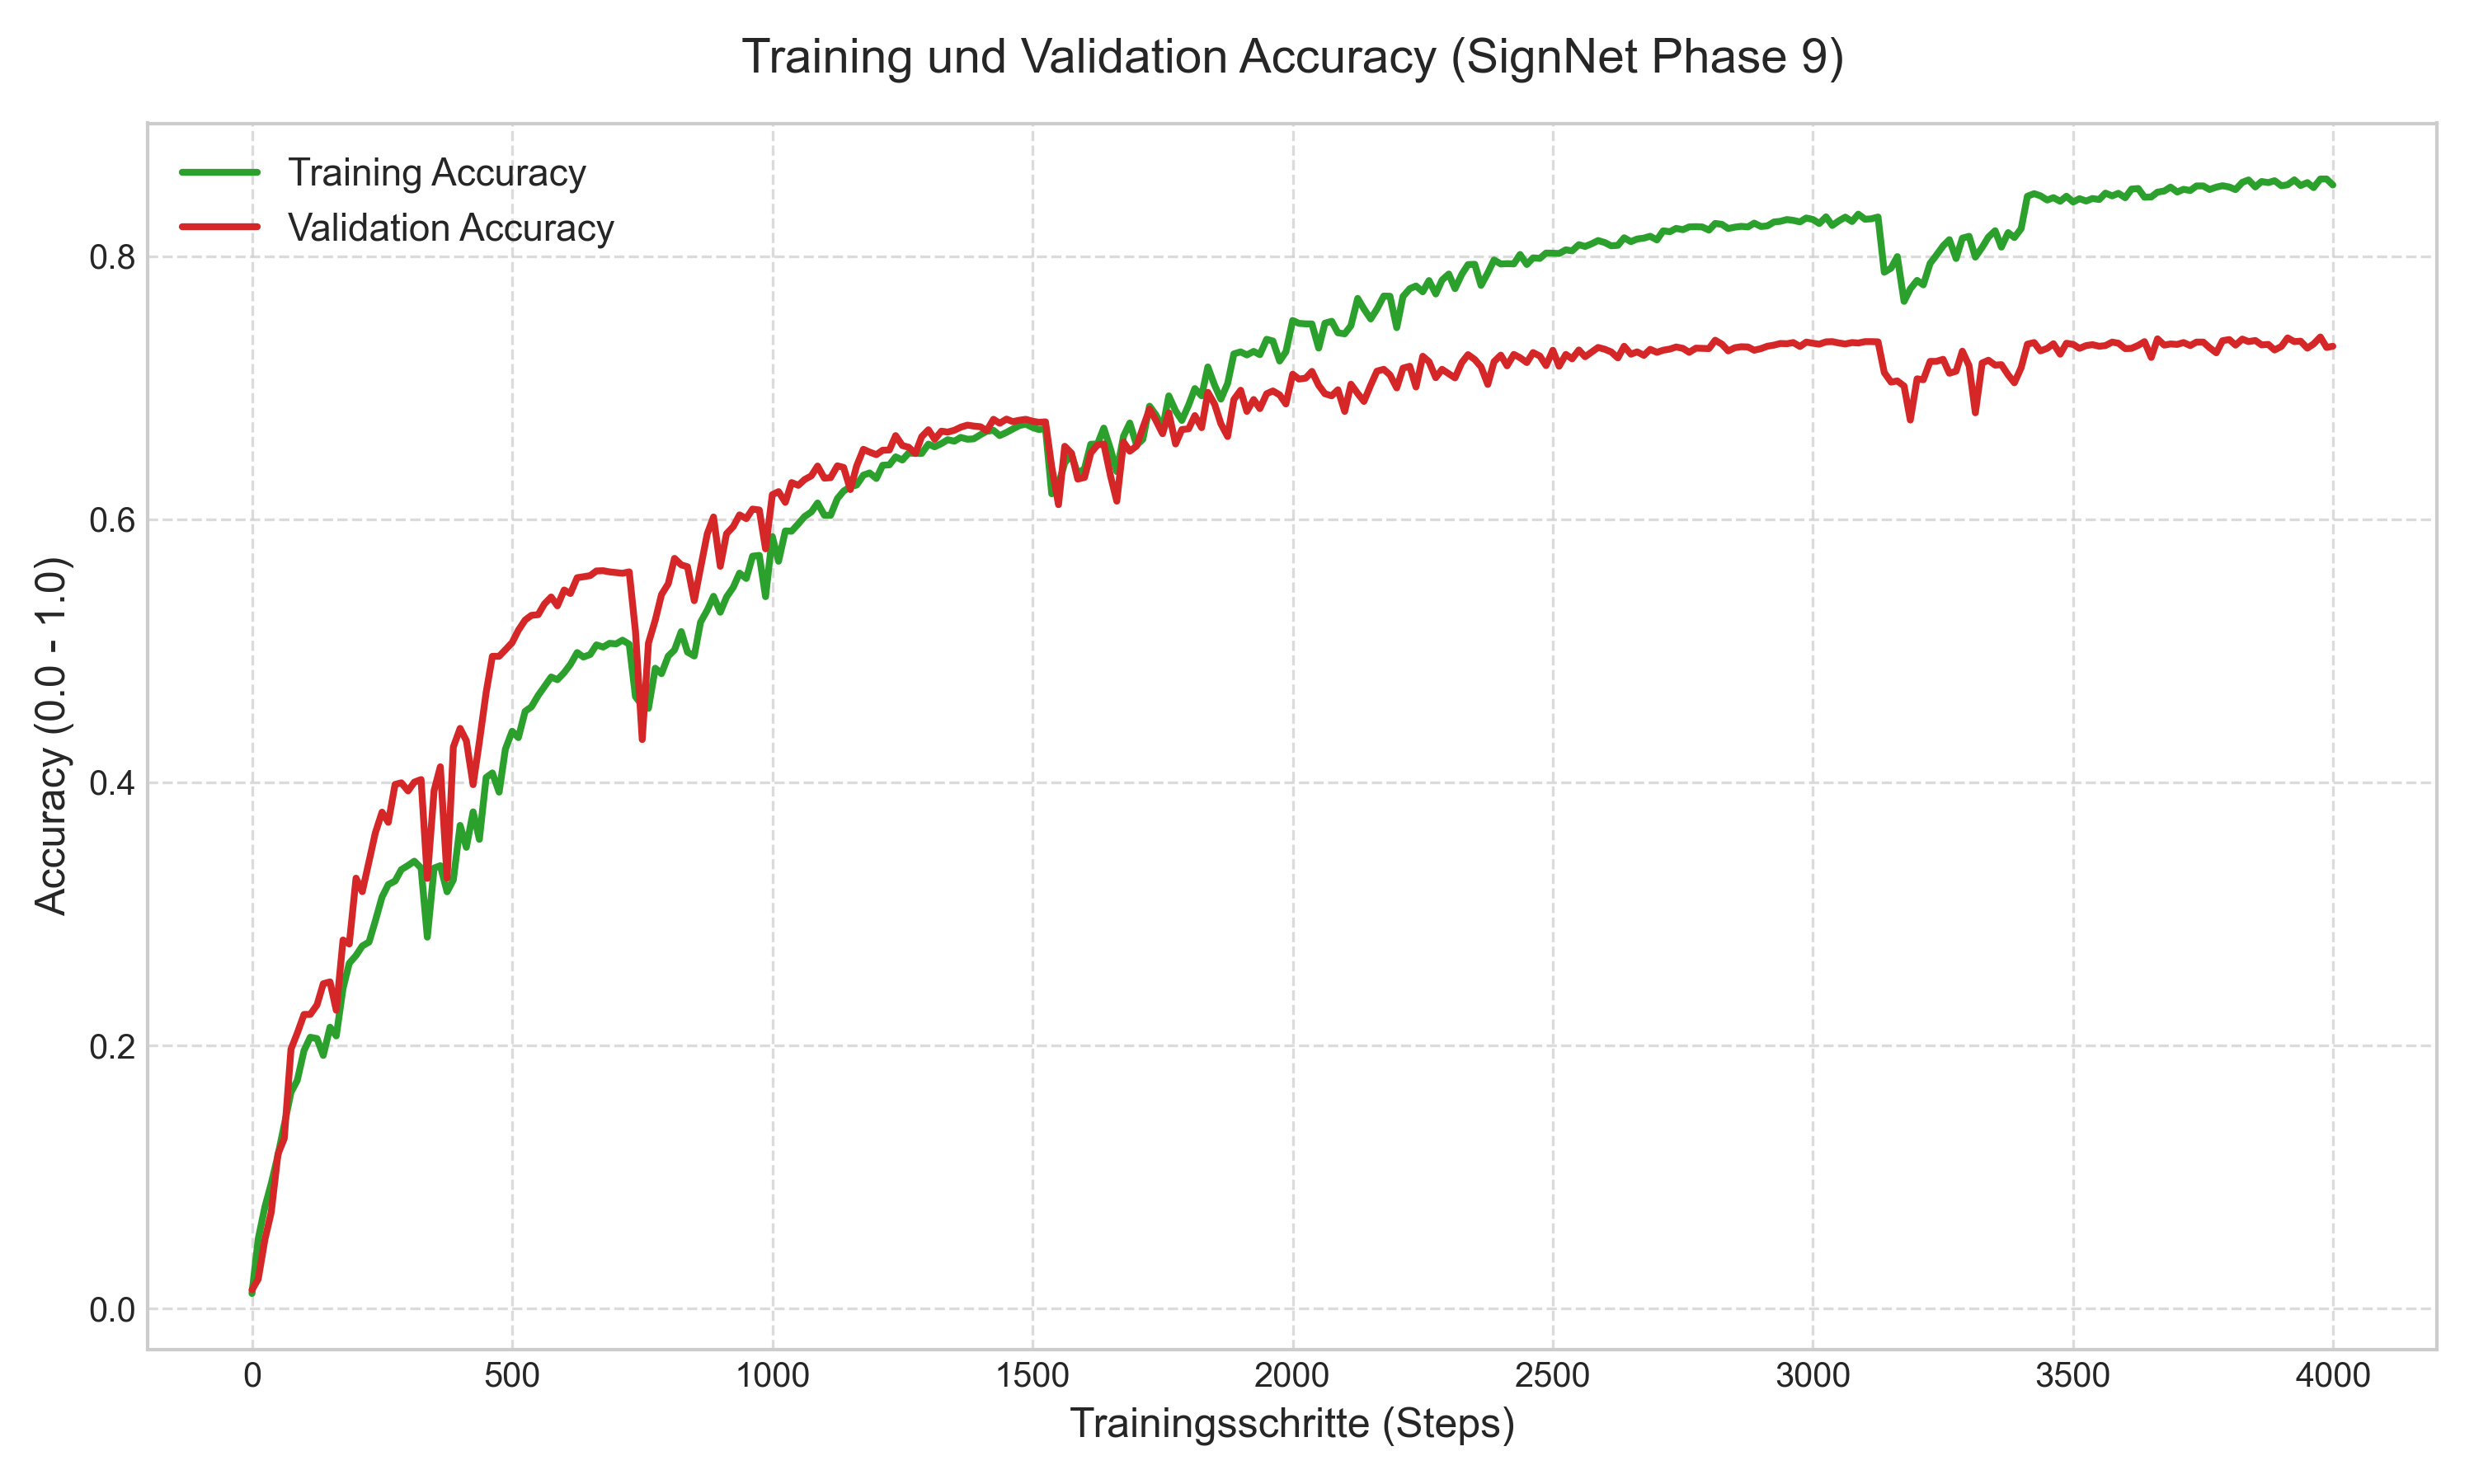
\includegraphics[width=0.85\textwidth]{figures/accuracy_plot_final.png}
    \caption{Entwicklung der Trainings- und Validierungs-Accuracy über die Trainingsschritte.}
    \label{fig:accuracy_plot}
\end{figure}

Wie in \autoref{fig:loss_plot} ersichtlich, konvergieren Trainings- und Validierungsverlust stabil. Die Accuracy (\autoref{fig:accuracy_plot}) steigt parallel an, wobei die geringe Differenz zwischen den Kurven die Wirksamkeit der gewählten Regularisierungsmaßnahmen (Dropout 0,65) bestätigt.

\section{Quantitative Ergebnisse}
Die Modellleistung wurde anhand der Top-1- und Top-5-Accuracy bewertet. Bei einem Vokabular von 146 Klassen haben wir folgende Werte erreicht:

\begin{table}[h]
\centering
\caption{Globale Klassifikationsergebnisse (Phase 5)}
\label{tab:globale_ergebnisse}
\begin{tabular}{lr}
\toprule
Metrik & Wert \\
\midrule
Top-1 Accuracy & \textbf{73,86 \%} \\
Top-5 Accuracy & \textbf{91,76 \%} \\
Anzahl Test-Samples & 4.489 \\
Klassenanzahl ($N \ge 70$) & 146 \\
\bottomrule
\end{tabular}
\end{table}

Die hohe Top-5-Genauigkeit von über 91\,\% zeigt, dass das System in den meisten Fällen die richtige Gebärde unter den wahrscheinlichsten Kandidaten identifiziert – ein wichtiger Aspekt für den praktischen Einsatz in interaktiven Übersetzungssystemen.

\section{Konfidenz-Analyse und Kalibrierung}
Zur Bewertung der Vorhersagezuverlässigkeit haben wir die Softmax-Konfidenz untersucht. Die Ergebnisse zeigen eine klare Trennung zwischen sicheren und unsicheren Vorhersagen:

\begin{table}[h]
\centering
\caption{Statistische Auswertung der Modell-Konfidenz}
\label{tab:konfidenz_stats}
\begin{tabular}{lr}
\toprule
Kategorie & Durchschnittliche Konfidenz \\
\midrule
Korrekte Vorhersagen & \textbf{87,37 \%} \\
Fehlklassifikationen & \textbf{57,19 \%} \\
\midrule
Anteil „Sichere Fehler“ (Konfidenz $> 0,8$) & 5,30 \% \\
\bottomrule
\end{tabular}
\end{table}

\begin{figure}[htbp]
    \centering
    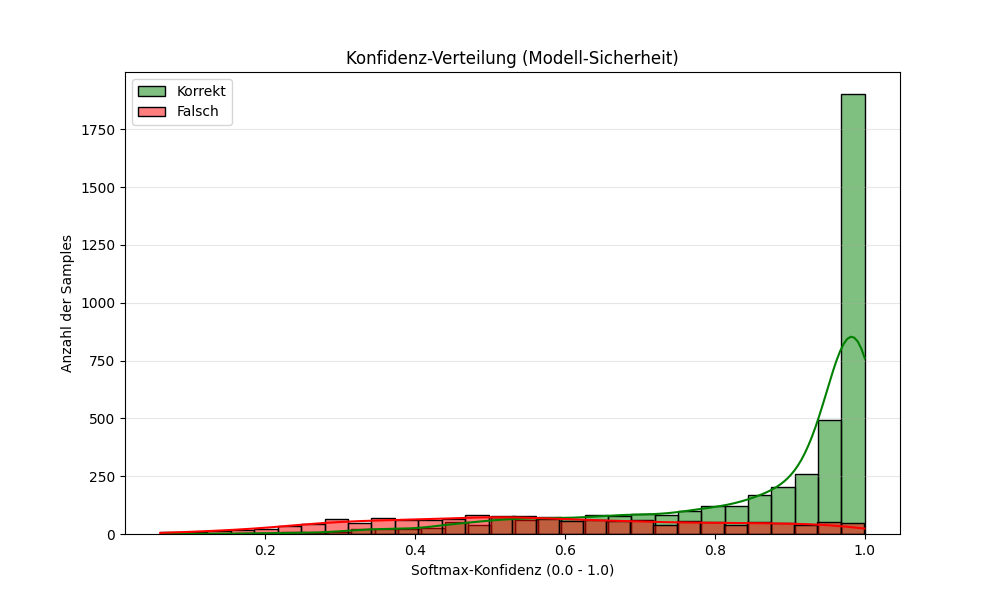
\includegraphics[width=1.0\textwidth]{figures/confidence_distribution.png}
    \caption{Konfidenz-Verteilung der Vorhersagen: Gegenüberstellung von korrekten (grün) und falschen (rot) Klassifizierungen zur Bewertung der Modell-Kalibrierung.}
    \label{fig:confidence_dist}
\end{figure}

Die Verteilung in \autoref{fig:confidence_dist} macht deutlich: korrekte Klassifizierungen liegen meist nahe bei 1,0, während Fehler deutlich unsicherer sind.

\section{Detaillierte Fehleranalyse}
Trotz der insgesamt robusten Performance gibt es systematische Verwechslungen. Die Konfusionsmatrix in \autoref{fig:confusion_matrix} zeigt die zehn Klassen mit dem niedrigsten F1-Score und dient als Grundlage für die linguistische Diskussion im nächsten Kapitel.

\subsection{Visualisierung der Fehlklassifikationen}
\autoref{fig:confusion_matrix} zeigt die Konfusionsmatrix für die 10 Klassen mit der geringsten Trennschärfe.

\begin{figure}[htbp]
    \centering
    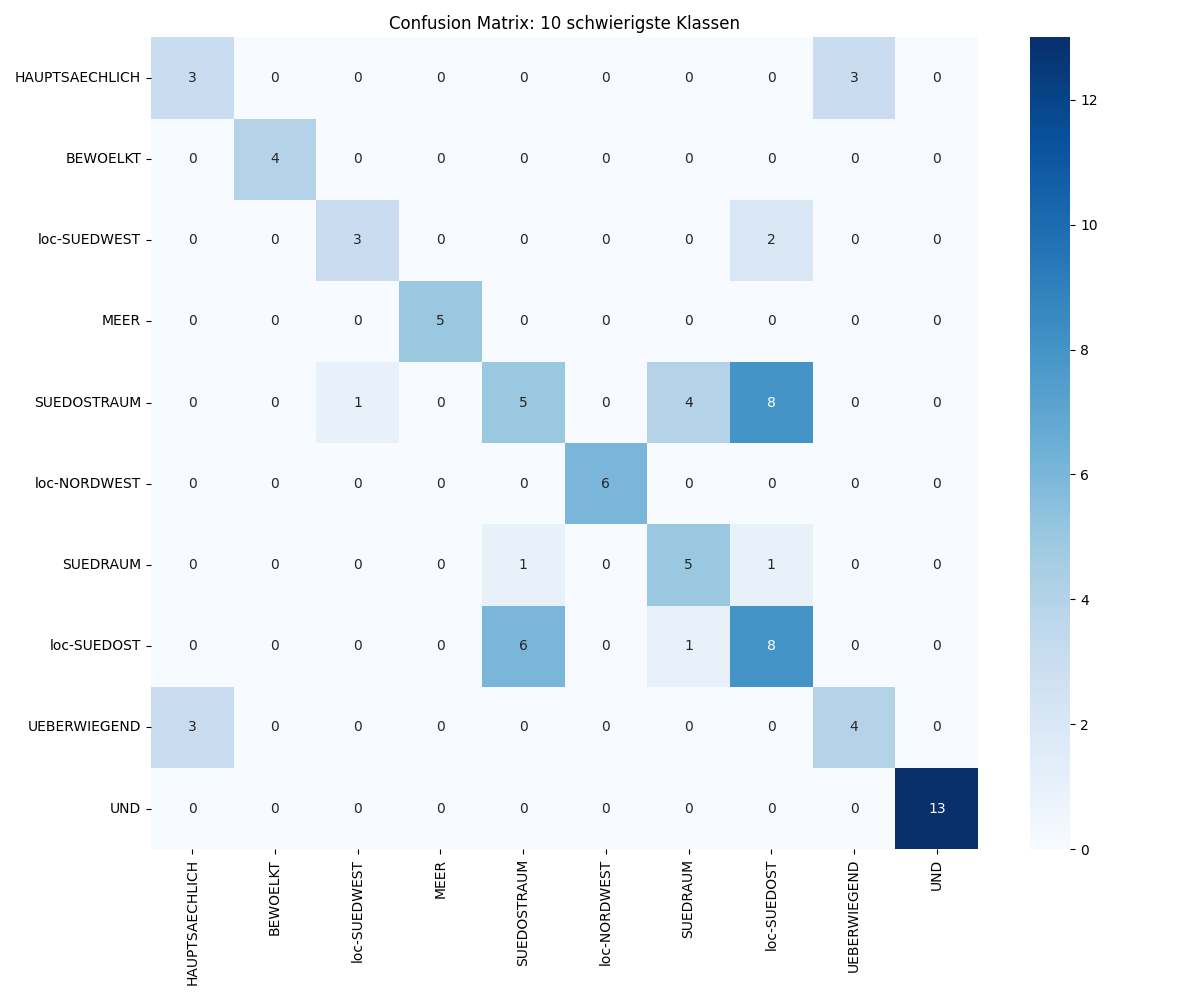
\includegraphics[width=1.0\textwidth]{figures/confusion_matrix_worst10.png}
    \caption{Konfusionsmatrix der 10 Klassen mit der geringsten Trennschärfe. Die Diagonale repräsentiert korrekte Vorhersagen, während die Nebenwerte die systematischen Verwechslungen innerhalb semantischer Gruppen visualisieren.}
    \label{fig:confusion_matrix}
\end{figure}
\chapter{Diskussion}
\label{ch:discussion}

In diesem Kapitel werden die Ergebnisse der finalen Phase 5 im Kontext der Forschungsfrage und der theoretischen Grundlagen interpretiert. Dabei wird die Brücke zwischen den rein statistischen Metriken aus Kapitel \ref{ch:results} und den linguistischen sowie architektonischen Herausforderungen geschlagen.

\section{Interpretation der Klassifikationsleistung}
Die finale Evaluation zeigt eine Top-1 Accuracy von 73,86\,\% auf einem Vokabular von 146 Klassen. Im Vergleich zur Baseline aus Phase 2 (53,94\,\%) belegt dies die signifikante Effektivität des optimierten Feature Engineerings und der finalen Transformer-Architektur. 

Besonders hervorzuheben ist die Top-5 Accuracy von 91,76\,\%. Diese Differenz von ca. 17 Prozentpunkten ist ein Indikator dafür, dass das Modell in über neun von zehn Fällen die korrekte Gebärde unter den wahrscheinlichsten Kandidaten identifiziert. Für die praktische Anwendung in einem interaktiven Assistenzsystem bedeutet dies eine hohe Resilienz, da die korrekte Information fast immer im engeren Auswahlfeld präsent ist.

\section{Analyse der Trainingsdynamik und Overfitting-Resilienz}
Ein zentraler Aspekt der Evaluation von Phase 5 ist die Untersuchung der Lernkurven im Hinblick auf die Generalisierungsfähigkeit des Modells und das Potenzial zur Trainingsoptimierung.

\subsection{Detaillierte Loss-Analyse}
Der Verlauf des \textit{Cross-Entropy Loss} liefert entscheidende Hinweise auf die Stabilität des Lernprozesses. Wie in Abbildung \ref{fig:loss_plot} ersichtlich, sinken sowohl der Training-Loss als auch der Validation-Loss über den gesamten Zeitraum stetig ab. 
\begin{itemize}
    \item \textbf{Konvergenzverhalten:} Beide Kurven erreichen gegen Ende der Trainingszeit ein stabiles Plateau, wobei der Training-Loss bei ca. 1,1 und der Validation-Loss bei ca. 1,55 stagniert. 
    \item \textbf{Fehlen von Divergenz:} Ein klassisches Anzeichen für Overfitting wäre ein Punkt, an dem der Validation-Loss wieder ansteigt, während der Training-Loss weiter sinkt. Da die Kurven im vorliegenden Experiment nahezu parallel verlaufen, kann eine destruktive Überanpassung an die Trainingsdaten ausgeschlossen werden.
\end{itemize}

\subsection{Interpretation des Accuracy-Gaps und Early Stopping}
Die Differenz zwischen der finalen Training-Accuracy (85,41\,\%) und der Validation-Accuracy (73,86\,\%) beläuft sich auf 11.55 Prozentpunkte. Eine zeitliche Analyse dieser Metriken offenbart jedoch ein signifikantes Optimierungspotenzial:

\begin{itemize}
    \item \textbf{Stagnation ab Schritt 2700:} Die Daten zeigen, dass die Validierungs-Genauigkeit bereits um Epoche 2700 einen Wert von ca. 73\,\% erreichte. In den verbleibenden 1300 Schritten verbesserte sich die Validierungs-Performance lediglich um marginale 0,8 Prozentpunkte, während die Training-Accuracy im selben Zeitraum von ca. 82\,\% auf ca. 85\,\% anstieg.
    \item \textbf{Reduzierung des Gaps:} Dieser Zuwachs der Training-Accuracy ohne entsprechende Verbesserung der Generalisierung ist ein Indikator für eine beginnende, wenn auch nicht kritische, Sättigung des Modells. Durch den Einsatz von \textit{Early Stopping} hätte das Training bereits bei Schritt 2700 beendet werden können. Dies hätte den finalen Generalization Gap von 11.55\,\% auf ca. 9\,\% reduziert, ohne dabei nennenswerte Einbußen in der Vorhersagegüte auf unbekannten Daten hinzunehmen.
    \item \textbf{Effizienz und Regularisierung:} Dass der Gap trotz des verzögerten Trainingsendes nicht weiter aufging, ist der starken Regularisierung (Dropout 0,65) zu verdanken, die eine stärkere Divergenz der Kurven erfolgreich unterdrückte.
\end{itemize}

\subsection{Zusammenfassende Bewertung der Generalisierung}
Trotz des Gaps von 11.55\,\% ist die Generalisierung als erfolgreich zu bewerten. Die parallelen Loss-Kurven beweisen, dass der Transformer robuste Repräsentationen gelernt hat, die über die reinen Trainingsbeispiele hinaus Bestand haben. Die Analyse legt jedoch nahe, dass für zukünftige Iterationen ein strikteres Early-Stopping-Kriterium die Trainingseffizienz steigern und die Differenz zwischen den Metriken weiter minimieren könnte.

\section{Detaillierte Analyse linguistischer Konfusionscluster}
Die Fehleranalyse in \autoref{fig:confusion_matrix} verdeutlicht, dass Fehlklassifikationen nicht zufällig auftreten, sondern systematischen linguistischen Mustern folgen:

\begin{itemize}
    \item \textbf{Morphologische Varianten und Classifier:} Die häufigsten Verwechslungen treten zwischen Stammgebärden und deren klassifikatorischen (\texttt{cl-}) oder lokalisatorischen (\texttt{loc-}) Erweiterungen auf. Die Paare \texttt{KOMMEN} vs. \texttt{cl-KOMMEN} (17 Verwechslungen) und \texttt{REGION} vs. \texttt{loc-REGION} (16 Verwechslungen) belegen, dass das Modell zwar die semantische Kernbewegung erkennt, jedoch Schwierigkeiten hat, die feinen räumlichen Nuancen im 3D-Raum der Landmarks exakt zu differenzieren.
    \item \textbf{Visuelle Minimalpaare:} Gebärden wie \texttt{ABEND} und \texttt{NACHT} (je 11 Fälle) oder \texttt{AUCH} und \texttt{ABER} (16 Fälle) teilen identische Handformen und Ausführungsorte. Die Unterscheidung basiert hier oft auf non-manuellen Markern (Mimik), die trotz Face-Mesh-Daten im Vergleich zur dominanten Handbewegung offenbar noch nicht ausreichend gewichtet werden.
    \item \textbf{Richtungskonfusion:} Die Verwechslung von \texttt{loc-NORD} mit \texttt{NORDRAUM} (15 Fälle) unterstreicht die Komplexität von Richtungsgebärden, bei denen sich die Trajektorien im PHOENIX-Kontext stark überschneiden.
\end{itemize}

\section{Modellstabilität und Konfidenz-Evaluation}
Die in Abbildung \ref{fig:confidence_dist} visualisierte Konfidenzverteilung liefert den Nachweis für eine erfolgreiche Modell-Kalibrierung.

\begin{itemize}
    \item \textbf{Trennschärfe:} Eine durchschnittliche Konfidenz von 87,37\,\% bei korrekten Vorhersagen gegenüber 57,19\,\% bei Fehlern belegt eine hohe Verlässlichkeit der Selbsteinschätzung des Systems. 
    \item \textbf{Vermeidung von Fehlentscheidungen:} Der geringe Anteil von 5,30\,\% an „sicheren Fehlern“ (Konfidenz $> 0,8$ bei falscher Vorhersage) ist ein starkes Indiz für die Robustheit der Architektur gegen das Auswendiglernen von Artefakten.
\end{itemize}

\section{Architektonische Einflüsse und Limitationen}
Der Erfolg von Phase 5 gegenüber den Vorphasen lässt sich auf die Rückkehr zur Transformer-Architektur mit einer kompakten \texttt{hidden\_size} von 256 Einheiten zurückführen. Während die Skeleton-Graphen in Phase 3 (31,56\,\% Accuracy) zu starr waren, erlaubt die Self-Attention des Transformers, zeitliche Abhängigkeiten über die gesamte Sequenz flexibel zu gewichten. 

Trotz dieser Fortschritte bleibt die phonologische Ähnlichkeit die größte Hürde. Die Ergebnisse legen nahe, dass zukünftige Iterationen eine noch stärkere Gewichtung von Mundbild-Features (Face-Mesh) innerhalb der Cross-Attention benötigen, um die verbleibenden Minimalpaar-Konfusionen weiter zu reduzieren.
\chapter{Fazit und Ausblick}
\label{ch:conclusion}

\section{Zusammenfassung der Ergebnisse}
Das Ziel dieser Arbeit war die Entwicklung und Evaluation eines robusten Systems zur isolierten Gebärdenspracherkennung unter Berücksichtigung extremer Klassenimbalance und visueller Ähnlichkeit. Mit dem Entwurf des \textit{SignNet}-Frameworks wurde eine Architektur implementiert, die einen Transformer-Encoder mit einem hierarchischen Experten-System kombiniert. Die Ergebnisse zeigen, dass die Basis-Genauigkeit von 52,34\,\% durch das gezielte Routing an spezialisierte Experten-Modelle auf 54,82\,\% gesteigert werden konnte. Dies belegt, dass eine hierarchische Unterteilung des Vokabulars in Konfusionsgruppen ein effektives Mittel zur Disambiguierung visuell ähnlicher Gebärden darstellt.

\section{Technische Würdigung}
Die technische Komplexität der Arbeit lag insbesondere in der Verarbeitung hochdimensionaler Landmark-Daten und der Bekämpfung von Overfitting bei gleichzeitigem Vorliegen eines "Long-Tail"-Datensatzes.
\begin{itemize}
    \item \textbf{Feature Engineering:} Die explizite Modellierung von Geschwindigkeit und Knochenvektoren erwies sich als entscheidend, um über statische Posen hinausgehende Bewegungsmuster zu erfassen.
    \item \textbf{Imbalance-Handling:} Durch den Einsatz von \textit{Balanced Softmax Loss} und \textit{Oversampling}-Strategien konnte eine stabilere Klassifizierung seltener Klassen erreicht werden, obgleich die Dominanz der "Head-Klassen" eine fundamentale Herausforderung bleibt.
    \item \textbf{Hierarchische Inferenz:} Das entwickelte System zur Inferenz-Steuerung erlaubt eine granulare Kontrolle über die Vorhersagequalität, stößt jedoch bei der automatischen Trigger-Logik ohne dediziertes Gating-Netzwerk an Effizienzgrenzen.
\end{itemize}

\section{Ausblick}
Zukünftige Forschungsansätze sollten die Integration von multimodalen Datenströmen (z.\,B. Kombination von Skelett-Daten mit optischem Fluss aus RGB-Videos) untersuchen, um die Erkennungsrate weiter zu stabilisieren. Zudem bietet die Erweiterung des hierarchischen Systems um ein lernbares Gating-Modell das Potenzial, die Routing-Präzision zu erhöhen und so die theoretische Performance der Experten-Modelle voll auszuschöpfen.

\section{Persönliches Fazit Andrei}
\label{sec:personal_conclusion_andrei}
Der Prozess der Erarbeitung dieser Abschlussarbeit war geprägt von der Auseinandersetzung mit realen, unvollständigen Daten und bot zahlreiche Lernmöglichkeiten. Im Folgenden reflektiere ich die Stärken, Verbesserungspotenziale und gewonnenen Erkenntnisse dieser Arbeit.

\subsection{Was habe ich gut gemacht?}
Die Projektarbeit hat mir gezeigt, dass systematisches Vorgehen der Schlüssel zum Erfolg ist. Besonders stolz bin ich auf die methodische Evolution des Projekts: Der Übergang vom statischen Fingeralphabet (99,6\,\% Accuracy auf 24 Gesten) zur kontinuierlichen Gebärdenerkennung auf dem RWTH-PHOENIX-2014 Datensatz war technisch anspruchsvoll, aber durch schrittweises Vorgehen beherrschbar.

Die \textbf{Datenanalyse vor architektonischen Entscheidungen} hat sich als goldrichtig erwiesen. Die systematische Untersuchung der MediaPipe-Landmarks zeigte beispielsweise, dass die Z-Koordinaten zu 80--98\,\% nahezu Nullwerte enthielten -- diese Erkenntnis ermöglichte eine Reduktion der Feature-Dimensionalität von 1'659 auf 1'086 Features ohne Performanceverlust.

Ein weiterer Erfolg war der \textbf{Umgang mit der extremen Klassenimbalance} (593:1 Ratio zwischen häufigster und seltenster Klasse). Die Implementierung von Balanced Softmax Loss in Kombination mit strategischem Oversampling für unterrepräsentierte Klassen führte zu einer Gesamtverbesserung von 11,4\,\% (67,16\,\% auf 78,54\,\% Accuracy). Besonders beeindruckend war die 18,2\,\%-Verbesserung bei Klassen mit weniger als 100 Samples.

Die Entwicklung eines \textbf{Bucket-basierten Evaluationssystems} -- inspiriert durch Feedback von Martin -- ermöglichte eine differenzierte Analyse der Modellperformance über verschiedene Sample-Strata hinweg. Dies half, gezielt Schwachstellen zu identifizieren und zu adressieren.

Schliesslich war die \textbf{konsequente Nutzung von MLflow} für Experiment-Tracking wertvoll. Die Dokumentation aller Hyperparameter, Metriken und Modell-Artefakte ermöglichte nicht nur Reproduzierbarkeit, sondern auch fundierte Entscheidungen für Folge-Experimente.

\subsection{Was würde ich anders machen?}
Die grösste Lektion kam durch einen schmerzhaften \textbf{Train/Inference-Mismatch}: Der Landmark-Extraktor für das Training nutzte separate MediaPipe-Modelle (Hands, Face, Pose) mit expliziter Handedness-Erkennung (LEFT immer auf Index 0--62, RIGHT auf 63--125), während die GUI-Demo MediaPipe Holistic mit einfacher Enumeration verwendete. Dieser fundamentale Unterschied führte dazu, dass das Modell im Demo-Modus praktisch blind war -- teilweise nur 14 von 94 Frames korrekt verarbeitete. Rückblickend hätte ich von Anfang an auf \textbf{konsistente Pipelines} zwischen Training und Inference achten müssen. Die Handedness-Erkennung hätte bereits in der ersten Iteration implementiert werden sollen, nicht erst nach Diagnose des Mismatch-Problems.

Auch beim Modell-Training gab es Lernmomente: Ein erster Optimierungsversuch mit erhöhter Regularisierung (Dropout 0,5, niedrige Learning Rate $5 \cdot 10^{-5}$) führte zu \textbf{Underfitting} statt der erhofften besseren Generalisierung -- der Validation Loss stieg von 2,89 auf 4,88. Die Balance zwischen Regularisierung und Model Capacity erfordert sorgfältige Abstimmung.

Im Rückblick würde ich der \textbf{initialen Datenbereinigung} und der Korrektur von Gloss-Label-Inkonsistenzen noch mehr Zeit widmen, da diese, wie auch in der Literatur beschrieben, die Basis für jede erfolgreiche Klassifizierung bilden. Eine zentrale Erkenntnis war, dass die Qualität der Vorverarbeitung (Landmark-Extraktion und Ausrichtung) oft einen grösseren Einfluss auf die finale Accuracy hat als die blosse Komplexität der Modellarchitektur.

Bei der \textbf{Dokumentation} hätte ich früher und kontinuierlicher arbeiten sollen. Die Thesis war zwar zu 70--80\,\% strukturiert, enthielt aber inkonsistente Accuracy-Zahlen zwischen verschiedenen Abschnitten -- ein Hinweis darauf, dass paralleles Schreiben und Experimentieren ohne strikte Synchronisation zu Inkonsistenzen führt.

\subsection{Was habe ich gelernt?}

\paragraph{Technisch}
Die Arbeit mit dem RWTH-PHOENIX-Datensatz vermittelte tiefgreifendes Verständnis für die Herausforderungen bei realen, unbalancierten Datensätzen. \textit{Balanced Softmax Loss} erwies sich als deutlich effektiver als simple Oversampling-Strategien allein -- die Kombination beider Techniken war der Schlüssel zum Erfolg.

MediaPipe ist ein mächtiges Tool, aber seine Nuancen -- insbesondere die unterschiedliche Handhabung von Handedness zwischen Holistic- und separaten Hand-Modellen -- erfordern genaues Studium. Die Erkenntnis, dass LEFT-Hände konsistent an definierten Indizes gespeichert werden müssen, war entscheidend für reproduzierbare Ergebnisse.

Die Transformer-Architektur mit 256 Hidden Units, 4 Layern und 4 Attention Heads ($\sim$4M Parameter) erwies sich als guter Kompromiss zwischen Performance und Overfitting-Risiko. Das ursprüngliche, grössere Modell (512h/6L/8heads, $\sim$21M Parameter) zeigte einen 16\,\%-Train/Validation-Gap.

Besonders lehrreich war zudem die Implementierung des \textit{MisclassificationAnalyzer}, der ein tiefes Verständnis für die semantische und visuelle Nähe von Gebärden ermöglichte.

\paragraph{Prozessbezogen}
Der wissenschaftliche Iterationsprozess -- Hypothese aufstellen, Experiment durchführen, Ergebnisse analysieren, Schlüsse ziehen -- ist keine abstrakte Methodik, sondern praktische Notwendigkeit. Die \glqq gescheiterten\grqq{} Experimente (V1 mit Overfitting, V2 mit Underfitting) waren keine Rückschläge, sondern lieferten wertvolle Erkenntnisse für die finale V3-Konfiguration.

Cross-Platform-Entwicklung zwischen Windows (Entwicklung) und Linux (vast.ai Training) erfordert sorgfältige Abstraktion von Pfaden und Konfiguration. Die Verwendung von \texttt{pathlib} und environment-aware Config-Klassen sparte später viel Debugging-Zeit.

\paragraph{Persönlich}
Das Projekt hat mir gezeigt, dass Machine Learning zu 80\,\% Data Engineering und Pipeline-Konsistenz ist, und nur zu 20\,\% Modell-Architektur. Diese Lektion werde ich in jedem zukünftigen ML-Projekt beherzigen.

\section{Persönliches Fazit Roman}
\label{sec:personal_conclusion_roman}
\subsection{Was habe ich gut gemacht?}
\subsection{Was würde ich anders machen?}
\subsection{Was habe ich gelernt?}

% You can divide your thesis into parts. If you want to, uncomment this line for the first part.
%\part{Einleitung}\label{partIntro}


% You can divide your thesis into parts. If you want to, uncomment this line for another part.
%\part{Tutorial}\label{partTutorial}




% ----- END OF THE MAIN BODY OF THE DOCUMENT -----

% ----- BEGIN OF THE APPENDICES -----
\appendix


% First we enumerate the most often used acronyms
%\chapter{Common Acronyms}\label{acronyms}

% You have to sort them manually

\begin{acronym}[JAX-RS]
\setlength{\itemsep}{-\parsep}
\acro{AJAX}{Asynchronous JavaScript And XML}
\acro{ANSI}{American National Standards Institute}
\acro{CERN}{European Organization for Nuclear Research}
\acro{CSS}{Cascading Style Sheet}
\acro{CGI}{Common Gateway Interface}
\acro{cURL}{Client for URL}
\acro{DBMS}{Database Management System}
\acro{DOM}{Document Object Model}
\acro{ERM}{Entity Relationship Model}
\acro{HL7}{Health Level 7}
\acro{HTML}{Hypertext Markup Language}
\acro{HTTP}{Hypertext Transfer Protocol}
\acro{HTTPS}{Hypertext Transfer Protocol Secure}
\acro{IANA}{Internet Assigned Numbers Authority}
\acro{IoT}{Internet of Things}
\acro{IP}{Internet Protocol}
\acro{IPSec}{Internet Protocol Security}
\acro{JAXB}{Java Architecture for XML Binding}
\acro{JAX-RS}{Java API for RESTful Web Services}
\acro{JPA}{Java Persistence API}
\acro{JPQL}{Java Persistence Query Language}
\acro{JSON}{JavaScript Object Notation}
\acro{JSP}{Java Server Pages}
\acro{JSTL}{Java Server Tag Library}
\acro{NCSA}{National Center for Supercomputing Applications}
\acro{PHP}{Hypertext Processor}
\acro{POJO}{Plain Old Java Object} 
\acro{POM}{Project Object Model}
\acro{QR}{Quick Response}
\acro{RFID}{Radio Frequency Identification}
\acro{REST}{Representational State Transfer}
\acro{ROA}{Resource Oriented Architecture}
\acro{SAX}{Simple API for XML}
\acro{SOA}{Service Oriented Architecture}
\acro{SQL}{Structured Query Language}
\acro{SPDY}{SPeeDY, an open networking protocol}
\acro{TCP}{Transmission Control Protocol}
\acro{URI}{Unified Resource Identifier}
\acro{URL}{Uniform Resource Locator}
\acro{VPN}{Virtual Private Network}	
\acro{W3C}{World Wide Web Consortium}
\acro{WADL}{Web Application Description Language}
\acro{WSDL}{Web Service Description Language}
\acro{WoT}{Web of Things}
\acro{XML}{eXtensible Markup Language}
\acro{XSD}{XML Schema Definition}
\end{acronym}


%\renewcommand*{\acsfont}[1]{\textbf{#1}}

% Here we include the licence of the paper. It is always the GNU Free Documentation License.
%\include{appendix/licence}

% This appendix gives the URL of the official web page of the present project
%\chapter{Website of the Project}\label{appendix_website}
A web-page was created for this project: \src{http://www.gmipsoft.com/rfid}\footnote{This URL is a shortcut to \url{http://diuf.unifr.ch/drupal/softeng/teaching/studentprojects/ehealth}}. On this page you will find:
\begin{itemize}
\item The API of the project.
\item This binaries and sources of this documentation.
\item The binaries and sources of the.
\item Parts of the content (see \ref{fig:cdrom}).
\end{itemize}
\ref{fig:official_website_fig} provides a screenshot of this website.

\begin{figure}[H]
\centering
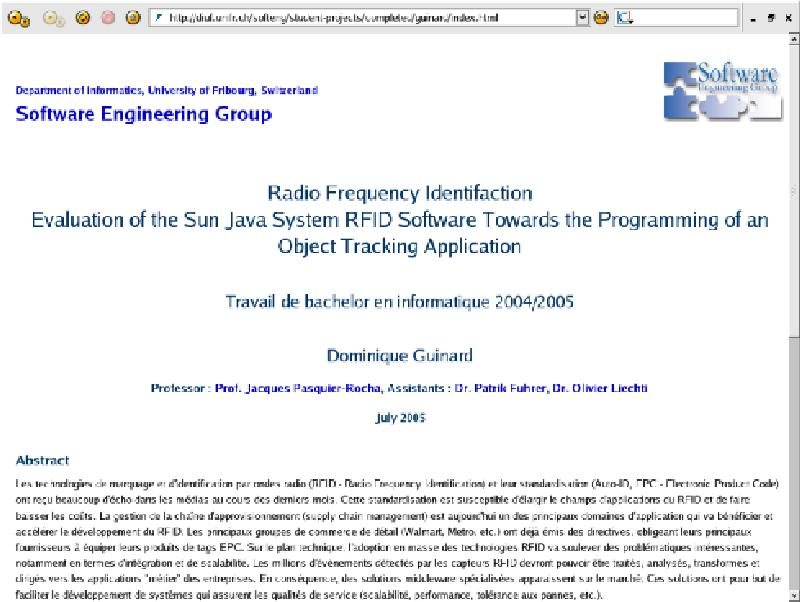
\includegraphics[width=\textwidth]{figures/official_webpage.jpg}
\caption{Screenshot of the project's official web-page}
\label{fig:official_website_fig}
\end{figure}



% This appendix contains the CDROM and briefly describes its content
%\chapter{CD-Rom}
\section*{Overview of the content}
\dirtree{%
.1 /.
.2 /ARC.
.2 /curl.
.3 /thesis\_commands.
.2 /eHealthServer.
.3 /\dots.
.2 /SQL.
.2 /XML.
}
\section*{Short description}
\textbf{ARC}
\par{
Contains a JSON formatted file, that can be imported as project in the Advanced Rest Client, a plugin for Chrome. It contains a full set of all possible resource operations for testing. 
}
\\\\
\textbf{curl}
\par{
Contains all files described in the appendix for the eHealthServer documentation.
}
\\\\
\textbf{eHealthServer}
\par{
Contains the latest snapshot of the eHealthServer taken on \today. It can be imported as is into Netbeans. 
}
\\\\
\textbf{SQL}
\par{
Contains the ERM file and a SQL dump file for a MySQL Server. 
}
\\\\
\textbf{XML}
\par{
Contains the WADL and XSD file. 
}
\\
\\
\begin{figure}[H]
\centering
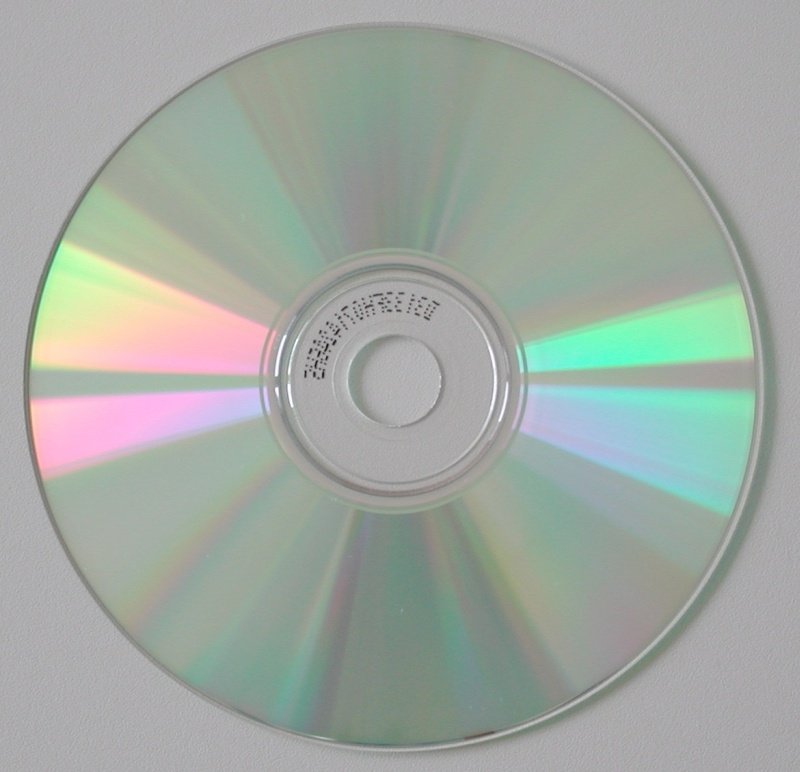
\includegraphics[width=\textwidth]{figures/cdrom.jpg}
\caption{The CD-ROM of this project}
\label{fig:cdrom}
\end{figure}



% The bibliography comes here, in alpha style.
% The title of bibliography is changed. Force it to be "References" instead of "Bibliography".
%\renewcommand{\bibname}{References}
\addcontentsline{toc}{chapter}{Literaturverzeichnis}
\bibliographystyle{plain}
\bibliography{mainbib}

%\renewcommand{\bibname}{Web Ressourcen}
%\addcontentsline{toc}{chapter}{Web Resourcen}
%\bibliographystyleweb{plain}
%\bibliographyweb{webbib}

\pagestyle{empty}
\printindex

% ----- END OF THE APPENDICES -----

\end{document}
% ***** END OF THE DOCUMENT *****
